\section{Models of Associative Memory}

Three models for associative memory are explored in this section, two traditional machine learning models and one emerging technology. While the traditional models (Hopfield networks and Boltzmann machines) may be considered abstract models defined independent of underlying hardware, they are in practise often employed on commodity hardware with a von-Neumann architecture. The emerging technology (memristors) however, enables a radically different computer architectures on top of which new models for associative memory (and other machine learning tasks) may be developed, and for which existing models may be ported to.

% === [ Subsections ] ==========================================================

\subsection{Hopfield Network}

\subsubsection{Implementation Example: Optical Information Processing}
In paper from D.Psaltis and N.Farhat(1985) \cite{optical_processing}, thresholding and feedback properties from Hopfield model was used in implementation of an optical system that processes optical information.

Enhanced error-correcting capability is one important outcome which is benefited from Nonlinearity of Hopfield model. With $M$ words of each binary vector $v_i$ with length of N bits, matrix $T_{ij}$ represents a storage of information. Matrix $T_{ij}$ gets multiplied by a stored binary vector $v'_i$ results in a \texttt{pseudoeigensystem} if $N$ is sufficiently larger than $M$. This indicated that the output vector $v''_i$ equals the input.

Supposed nonlinear iterative procedural experiments of certain number of known bits $N_1$ and the rest bits set to zero inside total of $N$ bits long vector were addressed to discover under what conditions the number of correct bits $N_2$ in output will be higher than $N_1$. A SNR(signal-to-noise ratio) equation which consists ratio of the expected value to the standard deviation on the same output vector, was used. As the Hopfield model has studied on the convergence property with respect to asynchronous operations, insensitivity to imperfections(nonuniformities, exact form of the threshold operation and errors in $T_{ij}$ matrix) and correct convergence obtained with thresholded $T_{ij}$. These all become most desired properties in optical implementation. Detailed optical implementation with 2D inputs was presented which was based on spatial-frequency multiplexing. Methods using Fourier transform, transmitting amplitude(weighted sum) and integral of the product of the input images were introduced in such an implementation. The robustness of a such system with nonlinear feedback becomes the most important feature.
As a conclusion, the implementation with the capabilities and limitations of optical techniques matches excellently with the Hopfield model that requires global, linear operations and local, point nonlinearities in a fully interconnected optical system.

\subsubsection{Memory Capacity with Modification: \\ replacing sigmoid neuron with a nonmonotonic neuron}
In paper from S.Yoshizawa, M.Morita and S.Amari(1992) \cite{capacity_of_nonmonotonic_model} it started with introduction of a new method by replacing sigmoid neuron with a nonmonotonic neuron and discussed theorectically on potential of absolute capacity(the maximum number of randomly generated patterns which are memorized as the equilibria of the network with the correlation-type connection weights) to be of order $n$ (nearly equal to $0.4n$).

Previous memory capacities were briefly introduced that Hopfield(1982) model's associative memory capacity is $0.15n$, the proven result of absolute capacity is asymptotically $ \frac{n}{2\log{n}} $ (from McEliece, Posner, Rodemich, \& Venkatesh, 1987; Weisbuch, 1985), and relative capacity(recalling process) is about 0.14n(with admission of small percent of errors) with replica method, but about $0.16n$ with a simply approximation method from respectively two different research work.

Various research suggestions were mentioned though all failed to deal completely with flaws of the conventional model, that both absolute and relative capacities are too small as well as the existence of large number of spurious memories. With a nonmonotonic neuron the result turned to be $0.4n$ for the absolute capacity which is even greater than relative capacity while the spurious memory disappeared.

With conventional neuron, memorized pattern is unstable, whereas a basin of attraction around memorized pattern was shown with nonmonotonic neuron by replacing sigmoid function with a nonmonotonic output function \textit{figure \ref{fig:nonmonotonic}} to neuron elements from the recalling process of an autocorrelation associative memory. This was named as Morita Model in the paper though it is essentially an extension from Hopfield Model.
By then the existence of equilibrium solutions and local stability, the authors did not further investigate on problems as the following: the size of the basin of attraction, the full sketch of spurious memories and the behaviour for clustered memorized patterns, which leaves more research work for future researchers to understand better associative memory with nonmonotonic neurons.

\begin{figure}[htbp]
	\centering
	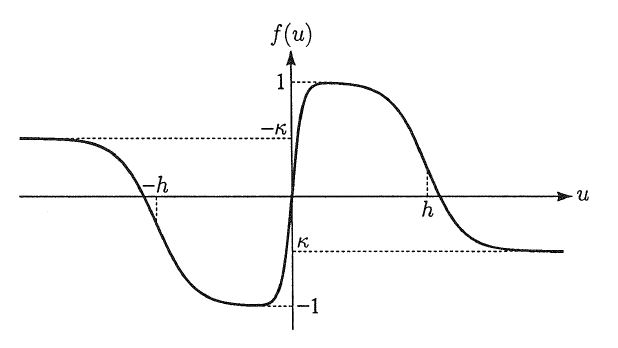
\includegraphics[scale = 0.8]{inc/nonmonotonic.jpg}
	\caption{The nonmonotonic output function, S.Yoshizawa, M.Morita and S.Amari(1992)}
	\label{fig:nonmonotonic}
\end{figure}

%THIS IS STH EXTRA OUTSIDE HOPFIELD
\subsection{Experiment on Implicit Memory for Novel Associations between pictures: \\ Effects of Stimulus Unitization and Aging}

From various previous research, concepts such as associative priming, unitization, difference between conceptual and perceptual associative priming, verbal versus pictorial material/stimuli and roll of spatial proximity were briefly summarized \cite{stimulus_unitization_and_aging}.

Experiments with pictorial stimuli(paired pictures) were done in 3 consecutive stages, where the result from first stage showed no evidence on requirement of spatial contiguity, though associative priming was enhanced compared to with spatially separated stimuli, which proved ``implicit memory for novel associations still can occur in the absence of an emergent conceptual representation''. The second experiment was an extension from the first experiment, with focus on the effects of aging and spatial contiguity of the same topic of stimuli on novel association priming between pictures, where stunning result was shown that ``associative priming is age invariant''(exposure of pictures was longer with older group to yield a matched performance in the baseline). The last experiment was based on both first and second experiments that ``associative priming with pictorial stimuli is modulated by spatial contiguity but not by aging'', and the study proved further evidence for the notion that novel association priming for picture pairs is mediated by the PRS(Perceptual Representation System).

%Wenting.

%1982, $0.15n$ (capacity of associative memory)
%
%% Above 0.15n releases the constraint on symmetries according to Olle.
%
%1985, proven $ \frac{n}{2\log{n}} $ (absolute capacity)
%
%1985, $0.14n$ (relative capacity of recalling process)
%
%1993, $ n ~= 0.4n $ (new result, absolute capacity)

\subsection{Boltzmann Machine}

% --- Lucas

\begin{figure}[htbp]
	\begin{center}
		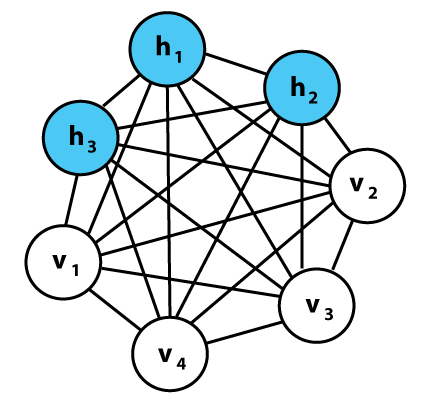
\includegraphics[width=0.5\textwidth]{inc/boltzmann_machine.png}
		\caption{Illustration of a Boltzmann Machine. The blue units represents three hidden units, while the four white units represents four visible units.\protect\footnotemark}
		\label{fig:boltzmann_machine}
	\end{center}
\end{figure}
\footnotetext{Original image (Public Domain): \url{https://en.wikipedia.org/wiki/File:Boltzmannexamplev1.png}}

The "Boltzmann Machine" (BM) is a form of "parallel constraint satisfaction network" \cite{ackley1985learning}. It is capable of learning the underlying constraints of a domain by only being shown examples of it. The BM is composed of units (also known as nodes) forming a complete graph where the connection between two units are symmetric; meaning that the weight on the connection is the same in either direction. No unit has a connection to itself. The units are binary, in the meaning that they can only assume one of two states, on or off. The state of a unit is determined by a probabilistic function based on the states of the units neighbours. A strong connection (high weight value) between two units indicates that if either of these two units are active, the other one should probably be active as well. While a weak connection (low weight value) indicates that these should probably not be active at the same time. This is analogous to Hebbian learning.

The BM is notably similar to the Hopfield network in that it also defines a global energy state of the system, utilizing the same equation that determines the global energy value. Each global state can be identified by the energy of the system in that state. By forcing the values of the visible units to represent a training set the system attempts to find an energy configuration that is compatible with the given input. The resulting energy state can then be interpreted as to how well the given data fulfils the constraints of the domain. Thus by minimizing the energy the system learns an interpretation of the problem that increasingly satisfies the constraints of the domain.

The simplest way to minimize the energy into a local minimum of the system is to change each units state into a value that results in a lower energy state. The data needed to determine this change is locally accessible to each unit, and is dependent on the current state of the units neighbours. If the sum of all values for a given units neighbour exceeds the threshold of that unit, the resulting state of the unit should be on. Otherwise it should be off. This is the usual algorithm for binary units.

Because of this deterministic algorithm it suffers from the usual weaknesses of gradient descent algorithms, namely, it gets stuck in local minima if its initial state is close to one. In order to alleviate the algorithm of this problem, noise is introduced in the training. This allows the network to "jump" out of these minima into configurations of higher energy. The algorithm used for noise introduction is a variation of the "Metropolis algorithm" \cite{metropolis1953equation} that was used to study thermodynamic systems. This modified version introduces a concept of temperature to the machine, which then tries to reach "thermal equilibrium" during training. Meaning that the machine is allowed to run repeatedly until the global energy of the system converges to a fixed state over a temperature that is initially high and then slowly decreased over the runtime of the system. The probability of finding the system in a global state after it has reached thermal equilibrium follows a Boltzmann distribution. If the temperature feed into the machine is equal to zero the stochastic nature of it is removed, the machine becomes deterministic and can be seen as a regular Hopfield network.

%TODO discuss the usage of hebbian learning in boltzmann
%TODO write more about this temperature thing
%TODO write more about the probabilistic features of the BM as well as the boltzmann distribution that gives the system its name.

Training is conducted in two phases, in the first phase the visible units of the machine are set to the values of the training set. In the next phase the machine is allowed to run freely, independent of the training set. The machine is iteratively switched between these two phases for the duration of the training until it reaches thermal equilibrium. The goal of the training is for the machine to be able to generate the input vector with a high probability of success.

% --- NOTES
%The difference between the BM and the Hopfield network is mainly that the nodes (or units as they are referred to in the original paper) of the Boltzmann Machine are stochastic by nature.
%The BM can be used for constraint satisfaction problems that involve a large amount of weak constraints.

\subsection{Memory Resistor}

%Robin.

In 2008, a group of researchers from HP labs published a paper entitled \textit{``The missing memristor found''} \cite{hp_memristor_found}. What, then, is a memristor, and how did we know it was missing? A memristor (short for memory resistor) is a resistor with memory whose resistance depends on the past flows of current passed through the circuit. The resistance of a memristor is increased by current travelling through it in one direction, and decreased by current travelling through it in the other direction. A memristor is a passive circuit which remembers its resistance even when inactive and without power for long periods of time. These properties make memristors interesting candidates for non-volatile storage and memory units, as they retain their state when unpowered, and specifically as they enable storage of continuous ranges of values (i.e. low \textit{through} high resistance) in contrast to discrete binary values (i.e. 0 \textit{or} 1).

Back in 1971, Leon Chua, often referred to as the father of non-linear circuit theory, laid the mathematical foundation detailing the relations between the four fundamental circuit elements. Interestingly, at that time only three fundamental circuit elements had physical counterparts, namely resistors, capacitors and inductors. The fourth fundamental circuit element, the memristor, was only conceptualized in theory by Chua for the sake of symmetry (see figure \ref{fig:circuit_elements}). As outlined in Chua's seminal paper \textit{``Memristor-the missing circuit element''} \cite{chua_memristor}, the current-$I$ voltage-$V$ curve of a memristor has a unique shape, an IV-fingerprint if you will, in the form of a pinched hysteresis loop (see figure \ref{fig:pinched_hysteresis}). A hysteresis loop indicates that a system has an internal state (i.e. memory) which affects the output of the system and which depends on past inputs to the system \cite{memristor_hayes}. As famously state by Chua, \textit{``If it's pinched it's a memristor''} indicates that the hysteresis loop passes through the origin.

% TODO: Explain the underlying reason of the hysteresis loop, i.e. alternating between two states (metastable switch).

\begin{figure}[htbp]
	\begin{center}
		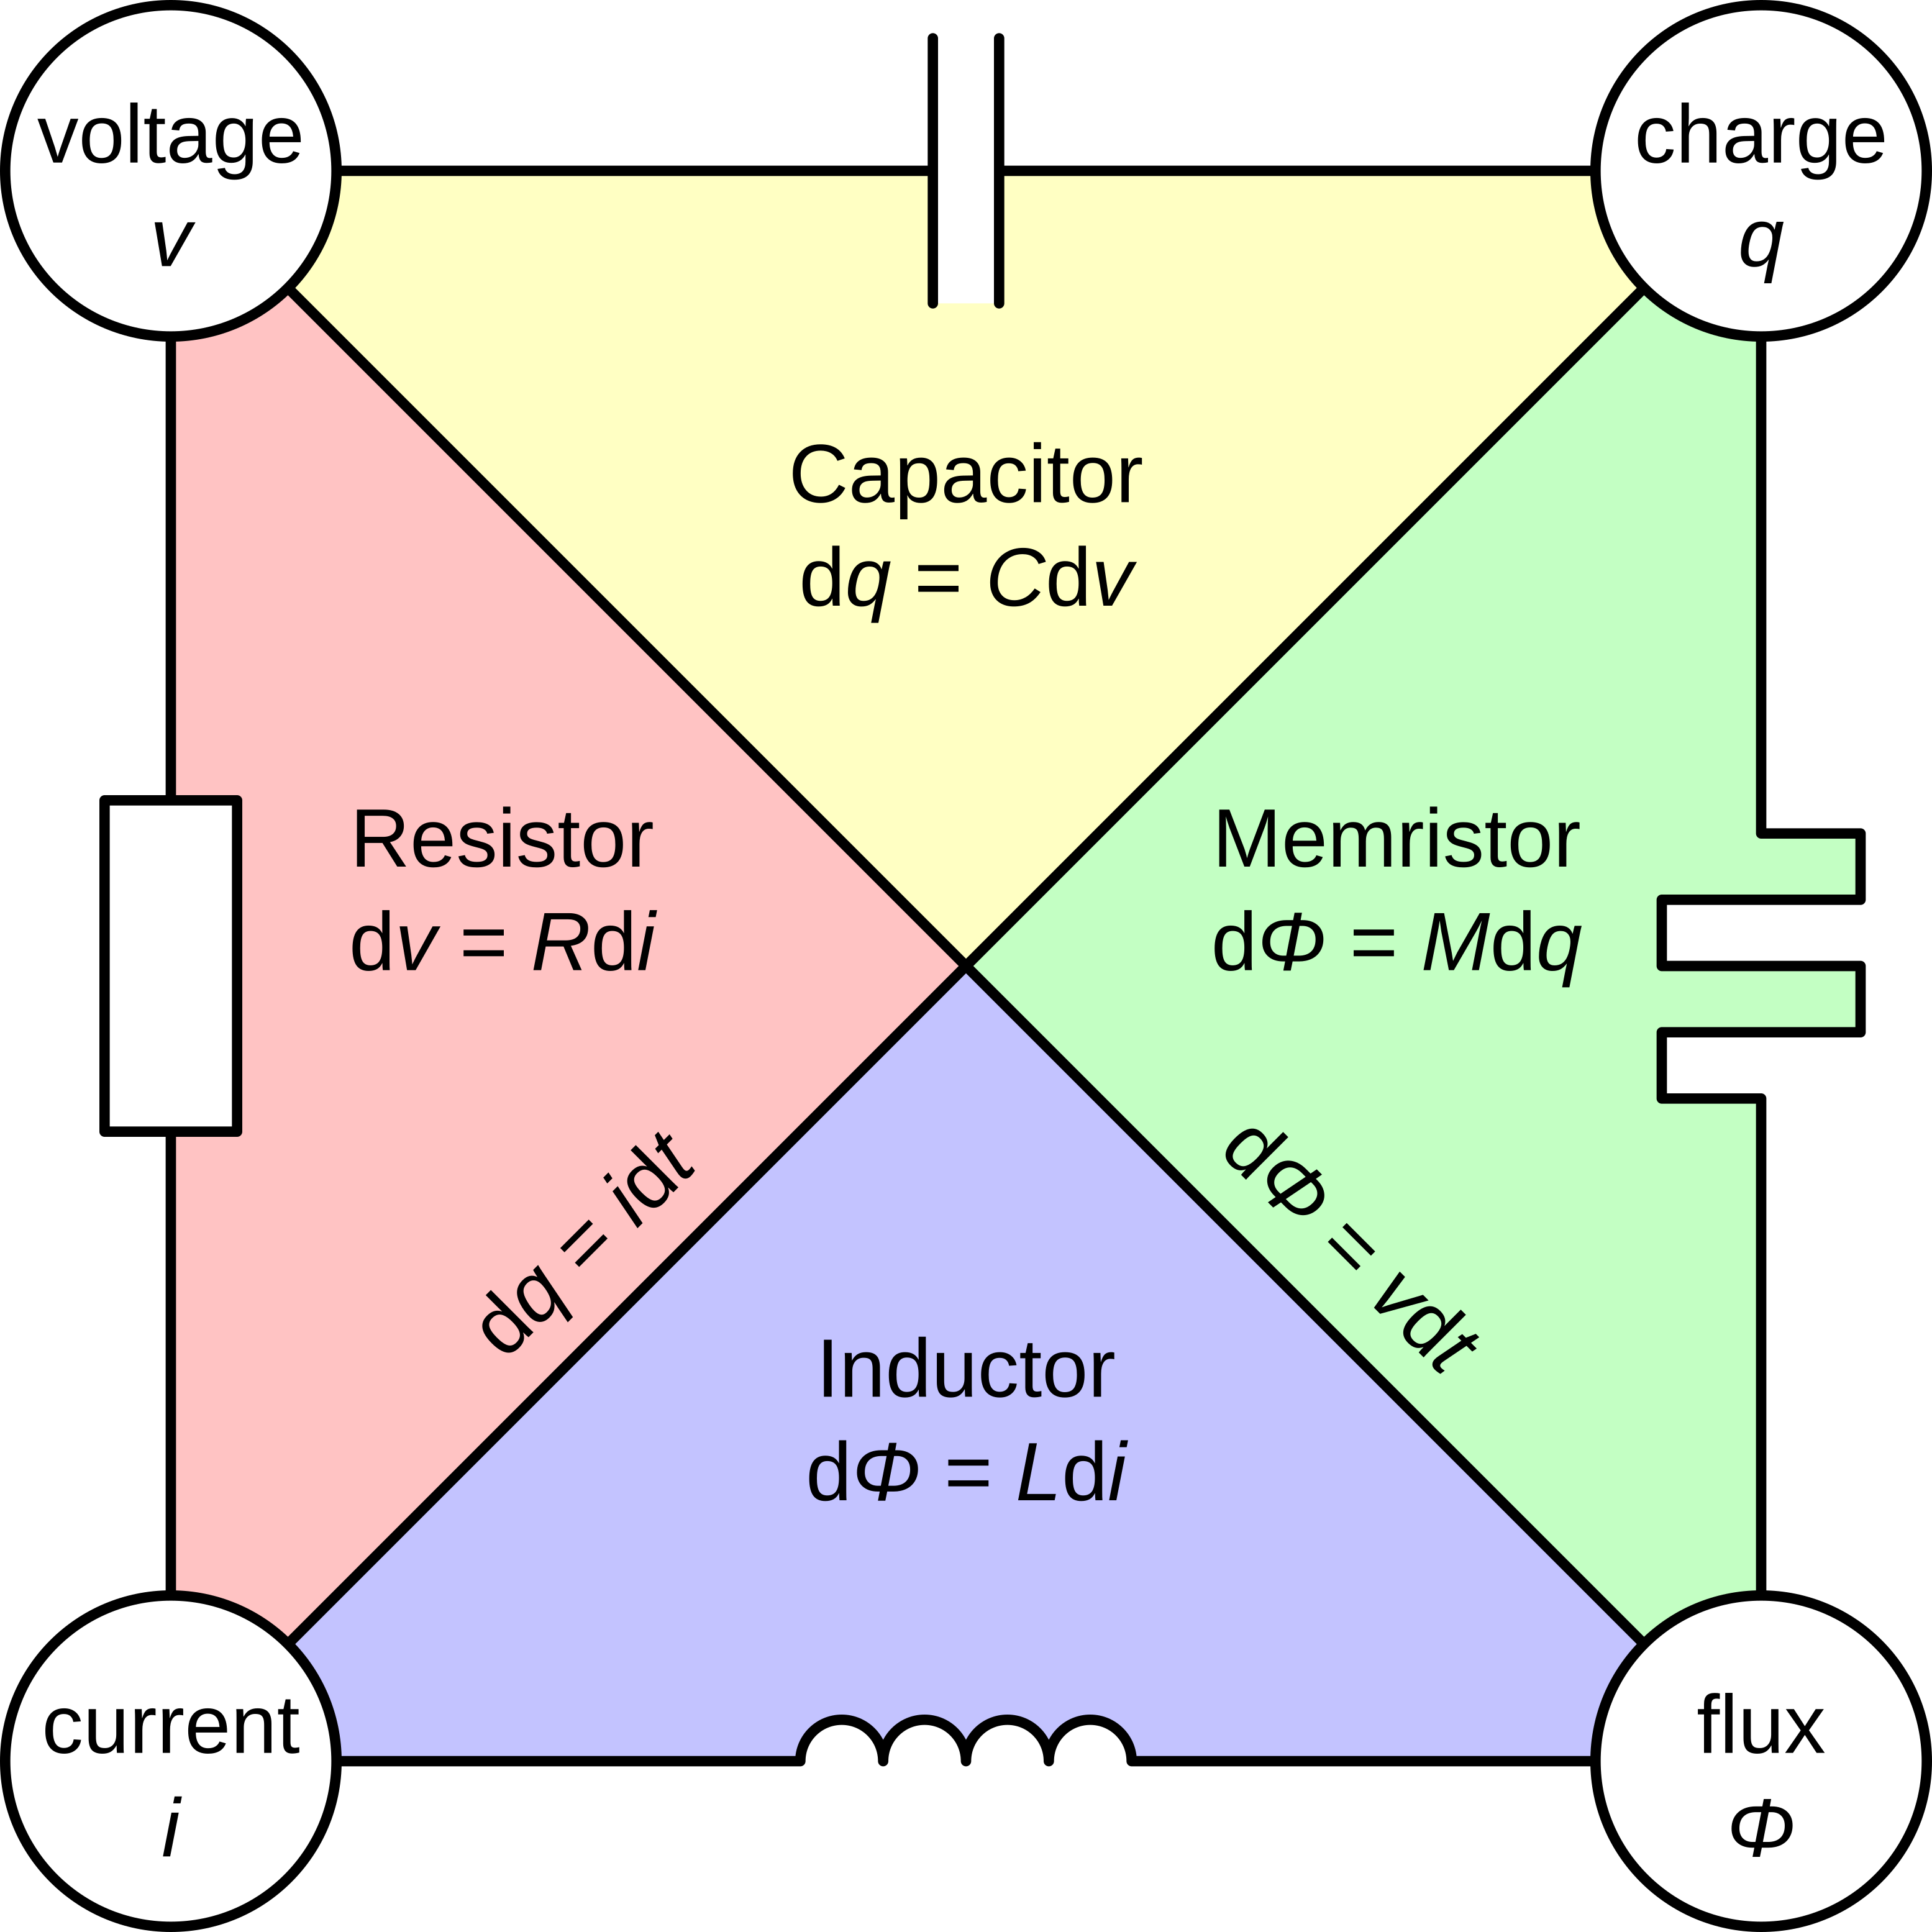
\includegraphics[width=0.5\textwidth]{inc/circuit_elements.png}
		\caption{Fundamental circuit elements.\protect\footnotemark}
		\label{fig:circuit_elements}
	\end{center}
\end{figure}
\footnotetext{Original image (CC BY-SA): \url{https://en.wikipedia.org/wiki/File:Two-terminal_non-linear_circuit_elements.svg}}

\begin{figure}[htbp]
	\begin{center}
		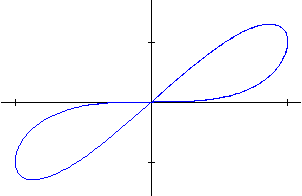
\includegraphics[width=0.5\textwidth]{inc/pinched_hysteresis.png}
		\caption{IV-curve of a memristor circuit, arrow indicates time.\protect\footnotemark}
		\label{fig:pinched_hysteresis}
	\end{center}
\end{figure}
\footnotetext{Original image (© Brian Hayes): \url{https://www.americanscientist.org/libraries/documents/201128120228377-2011-03CompScienceHayes.pdf}}

% TODO: Continue from here.

Several similarities have been identified between the properties of memristors and synapses, which make them interesting candidates for associative memory models; as further described in section \ref{sec:current_capabilities_memory_resistor}.

% ref: Tim Molter HiPeac Prague 2016 Memristor Keynote
%
% Denser memory, faster read and write, lower energy use, non-volatile, and may represent continuous (i.e. not 0 and 1).
%
% How do we reach the power efficiency of a brain. "Don't simulate a brain, build a brain"
%
% We need to build a brain where the distance between memory and computation is 0.
%
% 1 billion fold discrepancy between current machine learning platforms and biological brains.
%
% We can operate on very low voltages because of the read and write phases that constantly repair relevant state.

% ref: Knowm Collaborates with Kris Campbell at BSU
%
% Continuous value stored as resistance in a memristor. breaking outside of the 0 and 1 box.

% ref: http://knowm.org/
%
% > ## Modern computing
% >
% > Clear distinction between memory and processing.
% > Shuttle information back and forth.
% > Takes too long, requires too much energy.
% >
% > ## New paradigm of computing
% >
% > The act of accessing memory is the act of processing.

% ref: https://www.youtube.com/watch?v=Tb2E-t11OH4 ("What is AHaH Computing?")
%
% > Large scale adaptive learning systems, like brains.
% >
% > Bring memory and processing closer together. Parallel computing.
% >
% > Reduce or eliminate the energy normally associated with computing those functions.

% ref: https://www.youtube.com/watch?v=IVDRcV8XvlI ("What is an AHaH node?")
%
% > Two memristors competing with each other.
% >
% > A kT-bit (thermodynamic bit), a synapse consisting of two memristors.
% >
% > Look at the leaf of a plant. Energy dissipating system, constructed of many bifurcating channels. Every place where the energy flow splits, you have an AHaH node. You have two competing energy dissipating pathways.
% >
% > Nature is built of AHaH nodes.
% >
% > Understand how things self-organize.

% ref: https://www.youtube.com/watch?v=R7HxFhVQVr4 ("Why AHaH computing?")
%
% > Current digital computing platforms are billions of times less power and space efficient than biology (brains) for synaptic operations.
% >
% > It's physically not possible to reach biological level efficiency without significant changes in both architecture and technology.
% >
% > "GPU's will save us." `No they won't, they just suck less`
% >
% > If you insist on separating memory and computing, you won't even get close to the capacity of biology.
% >
% > Traditional computing would go an inch while biology is able to circle the world.
% >
% > Effective intelligence.

% ref: https://www.youtube.com/watch?v=YOKr8n6Juhs ("Why is AHaH computing so efficient?")
%
% > Communication is way faster in technology than biology. 1 sec football field, 1 sec 7 times around the world.
% >
% > Neuron body: 4000-100 000 nm
% > Synapses: 500 nm
% > Viruses: 400-40 nm
% > Transistor: 28 nm
% >
% > If faster and smaller, why so inefficient?
% >
% > Currents naturally sum. The values are reduced to specific resistances.
% >
% > Memristor
% >
% > Measures the combined current.
% >
% > Memristors can radically reduce total communication distance for some problems (not all).
% >
% > Reduce voltage makes a big impact, since it's the voltage squared.
% >
% > E=(C*V^2)/2
% >
% > biology: 0.065V
% > computer: 1.2 v (18x biology) 18^2 -> 324.
% >
% > Reduce the communication distance and voltage.

% ref: https://www.youtube.com/watch?v=ZBJX6zzwnRI ("The Adaptive power problem.")
%
% > Noise is everywhere.
% >
% > Noise margin (analogue vs. digital).
% >
% > The signal gets corrupted by the noise.
% >
% > Memristors. Two meta-stable switches. Potential energy that has to be overcome to have a transition.
% >
% > We want: Low power + adaptation ("ability to change")
% > But: Parts will constantly break (because of noise), decay, volatility
% > Consequently: We need a mechanism of repair.
% >
% > The Adaptive Power Problem
% > Low Power + Adaptation = Parts break
% >
% > Intelligence -> Learning -> Adaptation

% ref: https://www.youtube.com/watch?v=NO9kmqr8NLk ("The Adaptive Power Solution")
%
% > Intrinsic mechanism of repair; inherent.
% >
% > What if constant adaptation *is* the mechanism of repair?
% >
% > What is the "essential nature" of adaptation?
% >
% > When nature minimizes its potential energy, it also solves our problem."; e.g. minimal surface with soap bubbles.
% >
% > To repair yourself is to be alive. Death is decay.
% >
% > Bejan (Construcal Law):
% > "For a finite-size system to persist in time (to live), it must evolve in such a way that it provides easier access to the imposed currents that flow through it."
% >
% > Swenson:
% > "A system will select the path or assembly of paths out of available paths that minimizes the potential or maximizes the entropy at the fastest rate given the constraints."
% >
% > England:
% > "Dissipation-driven adaptation of matter."
% >
% > E.g. The system will go with the flow, and it will maximize the flow.
% >
% > Maximize the dissipation of energy. The system will evolve in time towards that maximum, intrinsic repair.
% >
% > Have the system evolve itself to solve our problems.
% >
% > AHaH circuit. An intrinsic adaptation mechanism. Energy dissipation pathways competing for conduction resources.
% >
% > Everywhere in nature. Competing energy dissipating pathways. Fractal.
% >
% > A memristor is effectively an adaptive energy dissipating pathway. It's like a riverbed. As you pass current through it, it will change its resistance, the riverbed will get bigger. Make memristors compete for energy dissipation.
% >
% > AHaH - Anti-Hebbian and Hebbian plasticity
% >
% > "Maximization of energy dissipation" - Swenson
% > "Maximization of currents" - Bejan
% > "Dissipation-driven adaptation of matter" - England
% > "Energy dissipation pathways competing for conduction resources" as a mechanism.

% ref: https://www.youtube.com/watch?v=CFSrC7kjbJo ("Introduction to AHaH Computing, Alex Nugent, RIT, April 2015")
%
% > Focuses on self-organizational building blocks.
% >
% > Points of bifurcation, branches.
% >
% > Energy dissipating fractal pattern.
% >
% > d (the distance) is zero in the brain, has tremendous effects on energy usage.
% >
% > A memristor for each pathway, and they are competing with each other so you need two per synapse. Think of the pair as a synapse itself, and the different in conductance between the two is the value of the synapse. If one is more conductive than the other it is positive, and vice versa, its negative.
% >
% > Naturally they go towards zero. But if you give them a burst, you can make them positive or negative as you want. Read brings it a little closer together, then reward it.
% >
% > Hebbian (erase the path): Any modification to the synaptic weight that reduces the probability the synaptic state will remain upon subsequent measurement.
% >
% > Anti-Hebbian (select the path): Any modification to the synaptic weight that increases the probability the synaptic state will remain the same upon subsequent measurement.
% >
% > XXX [ IMPORTANT ] XXX
% >
% > Synaptic access is processing is adaptation (memory and processing merged, d=0).
% >
% > XXX [/ IMPROTANT ] XXX
% >
% > A neuron is this decision making thing. We are finding the decision boundary, a representation of the weights w_0, w_1.
% >
% > Maximize the classification margin.
% >
% > Opposing data distribution (energy dissipation pathways)
% > fight for classification margin (compete for conduction resources)
% >
% > Spike encoding (optic nerve). Which spikes within the spike space are active.
% >
% > FF-RF (forward-float, reverse-float), that is the as close to non-destructive read as you get. Reading is adaptation, it changes the memory.
% >
% > We can go backwards, discretized by the spikes.
% >
% > Nature has a universal adaptive building block.
% >
% > Interacting collectives of this building block solves the problems that the brain solves.
% >
% > memristors empower (not replace) our digital computers.

% ref: https://youtu.be/dgbooumJ4Tg?t=1692
%
% Won a nobel price. Eliol Prigoge.
% There is a natural tendency for complex systems to minimize the energy consumption

% === [ Knowm Synapses ] ===

%\subsubsection{AHaH Nodes}
%\subsubsection{Knowm Synapses}

% ref: http://knowm.org/knowm/
%
% A memristor is the electronic equivalent of an adaptive container!
%
% “Anti-Hebbian and Hebbian” in honour of Donald O. Hebb
%
% “Knowm's Synapse” or “Nature’s Transistor”. Two competing energy dissipation pathways.
%
% As a voltage (pressure) is applied to a memristor, its conductance will change.
%
% It is responsible for most self-organization on this planet. Nature is built of Knowms, including you.
%
% It is created when two energy dissipation pathways are competing for conduction resources. It appears to be at the heart of most self-organization.
%
% Knowm is built of a simple part repeated over and over again.
%
% When energy (for example water) flows through an adaptive container (for example dirt), the medium adapts or erodes in a particularly way that causes the energy to be dissipated faster. For example, the water erodes the ground and causes a channel to grow, which lowers the resistance to flow.
%
% ref: http://knowm.org/knowm-api/
%
% Every modern computing system currently separates memory and processing. This works well for many tasks, but it fails for large-scale adaptive systems like brains or large ML models like neural networks. Indeed, there is no system in Nature outside of modern human digital computers that actually separates memory and processing, so it’s a wonder we have been able to do as much as we have.

% ref: ref: http://knowm.org/report-from-the-navy-karles-invitational-on-neuro-electronics/
%
% Where each operation results in Anti-Hebbian or Hebbian learning. At the lowest level, Anti-Hebbian just means “move the synapse toward zero” and Hebbian means “move it away from zero”.

